\documentclass[12pt]{scrartcl}

\usepackage[T1]{fontenc}
\usepackage[utf8]{inputenc}
\usepackage{amsmath}
\usepackage{amsfonts}
\usepackage{amssymb}
\usepackage{amsbsy}
\usepackage{graphicx}
\usepackage{float}
\usepackage{array}
\usepackage{booktabs}
\usepackage{multirow}
\usepackage{bm}
\usepackage{verbatim}
\usepackage[english]{babel}
\usepackage{color}
\usepackage{url}
\usepackage{fancybox}
\usepackage[stable]{footmisc}
\usepackage[format=plain,labelfont=bf]{caption}
\usepackage{fancyhdr}
\usepackage{natbib}
\usepackage{calc}
\usepackage{textcomp}
\usepackage[pdftex,pdfborder={0 0 0}]{hyperref}
\usepackage{pdfpages}
\usepackage{tikz}
\usetikzlibrary{shapes,arrows,decorations.pathmorphing}

\renewcommand*{\familydefault}{\sfdefault}

% Margins
\addtolength{\textheight}{1.0cm}
\addtolength{\oddsidemargin}{-0.5cm}
\addtolength{\evensidemargin}{-0.5cm}
\addtolength{\textwidth}{1.0cm}
\parindent=0em

% New math commands
\newcommand{\overbar}[1]{\mkern 1.5mu\overline{\mkern-1.5mu#1\mkern-1.5mu}\mkern 1.5mu}
\DeclareMathOperator{\diag}{diag}
\DeclareMathOperator{\Diag}{Diag}
\DeclareMathOperator{\tr}{tr}
\DeclareMathOperator{\Cov}{Cov}
\DeclareMathOperator{\Cor}{Cor}
\newcommand\independent{\protect\mathpalette{\protect\independenT}{\perp}}
\def\independenT#1#2{\mathrel{\setbox0\hbox{$#1#2$}%
\copy0\kern-\wd0\mkern4mu\box0}} 

% Appropriate font for \mathcal{}
\DeclareSymbolFont{cmmathcal}{OMS}{cmsy}{m}{n}
\DeclareSymbolFontAlphabet{\mathcal}{cmmathcal}

% Set subscript and superscripts positions
\everymath{
\fontdimen13\textfont2=5pt
\fontdimen14\textfont2=5pt
\fontdimen15\textfont2=5pt
\fontdimen16\textfont2=5pt
\fontdimen17\textfont2=5pt
}

% Bibliography style
\setlength{\bibsep}{1pt}

% Part
\renewcommand\partheadstartvskip{\clearpage\null\vfil}
\renewcommand\partheadmidvskip{\par\nobreak\vskip 20pt\thispagestyle{empty}}
\renewcommand\partheadendvskip{\vfil\clearpage}
\renewcommand\raggedpart{\centering}

\begin{document}
\title{Multivariate localization}
\author{Benjamin Ménétrier}
\date{Last update: \today}

\thispagestyle{empty}

\maketitle
\begin{center}
Documentation for the code "BUMP", distributed under the CeCILL-C license.\\
Copyright \copyright 2015-... UCAR, CERFACS, METEO-FRANCE and IRIT
\end{center}

\tableofcontents

\clearpage


\section{Framework}

\subsection{Blocks definition}
A localization matrix $\mathbf{L} \in \mathbb{R}^{n \times n}$ is applied to a multivariate state vector $\mathbf{x} \in \mathbb{R}^n$, built as the concatenation of $p$ sub-vectors:
\begin{align}
\mathbf{x} = \left( \begin{array}{c}
\mathbf{x}_1 \\[1ex]
\hline
\vdots \\
\hline
\mathbf{x}_p
\end{array} \right)
\end{align}
where $\mathbf{x}_i$ is the sub-vector for variable $i$, of size $n_i$ with $\displaystyle n = \sum_{i=1}^p n_i$.\\
$  $\\
The localization matrix is split into blocks:
\begin{align}
\mathbf{L} = \left( \begin{array}{ccc}
\mathbf{L}_{11} & \cdots & \mathbf{L}_{1p} \\
\vdots & \ddots & \vdots \\
\mathbf{L}_{p1} & \cdots & \mathbf{L}_{pp}
\end{array} \right)
\end{align}
The main issue is to design a positive semi-definite localization matrix, and the simple solution is to build it as:
\begin{align}
\mathbf{L} = \mathbf{UU}^\textrm{T}
\end{align}
where $\mathbf{U} \in \mathbb{R}^{n \times m}$ is called a ``square-root'' of the localization matrix $\mathbf{L}$. The control vector $\mathbf{v} \in \mathbb{R}^m$ is such that:
\begin{align}
\mathbf{x} = \mathbf{U} \mathbf{v}
\end{align}

\subsection{Shared blocks}
For the case where several variables share the same localization, the $p$ variables are split into $q$ groups of sizes $p_1$ to $p_q$, with $\displaystyle \sum_{\alpha=1}^q p_\alpha = p$. The mapping between variables and groups is given by $\alpha = G(i)$, where $\alpha$ is the group index and $i$ the variable index. For sake of simplicity, we assume that variables are reordered so that the sub-vectors of a given group are contiguous:
\begin{align}
\mathbf{x} = \left( \begin{array}{c}
\widehat{\mathbf{x}}_1 \\[1ex]
\hline
\vdots \\
\hline
\widehat{\mathbf{x}}_{q}
\end{array} \right)
\end{align}
where:
\begin{align}
\widehat{\mathbf{x}}_\alpha = \left( \begin{array}{c}
\mathbf{x}_{\sum_{i=1}^{\alpha-1} p_i+1} \\[1ex]
\hline
\vdots \\
\hline
\mathbf{x}_{\sum_{i=1}^\alpha p_i}
\end{array} \right)
\end{align}

\section{Column square-root}
In this section, the localization square-root $\mathbf{U}$ is built as a column of matrices.

\subsection{Common block}
The simplest method defines $\mathbf{U}$ as:
\begin{align}
\mathbf{U} = \left( \begin{array}{c}
\overbar{\mathbf{U}} \\
\vdots \\
\overbar{\mathbf{U}}
\end{array} \right) = \left( \begin{array}{c}
\mathbf{I}_{\overbar{n}} \\
\vdots \\
\mathbf{I}_{\overbar{n}} \\
\end{array} \right) \overbar{\mathbf{U}}
\end{align}
where $\overbar{\mathbf{U}} \in \mathbb{R}^{\overbar{n} \times \overbar{m}}$ is the common square-root and $\mathbf{I}_{\overbar{n}} \in \mathbb{R}^{\overbar{n} \times \overbar{n}}$ is the identity matrix. The resulting localization matrix is:
\begin{align}
\mathbf{L} = \mathbf{U} \mathbf{U}^\mathrm{T} = \left( \begin{array}{ccc}
\overbar{\mathbf{U}} \overbar{\mathbf{U}}^\mathrm{T} & \cdots & \overbar{\mathbf{U}} \overbar{\mathbf{U}}^\mathrm{T} \\
\vdots & \ddots & \vdots  \\
\overbar{\mathbf{U}} \overbar{\mathbf{U}}^\mathrm{T} & \cdots & \overbar{\mathbf{U}} \overbar{\mathbf{U}}^\mathrm{T}
\end{array} \right)
\end{align}
In this case, each auto- or cross-localization block is given by: 
\begin{align}
\mathbf{L}_{ij} = \overbar{\mathbf{U}} \overbar{\mathbf{U}}^\mathrm{T}
\end{align}
\textbf{Control vector size:} $\displaystyle m = \overbar{m}$.\\
\textbf{Cost:} one application of $\overbar{\mathbf{U}}$.

\subsection{Specific blocks}
A third method defines $\mathbf{U}$ as:
\begin{align}
\mathbf{U} = \left( \begin{array}{c}
\overbar{\mathbf{U}}_1 \\
\vdots \\
\overbar{\mathbf{U}}_p
\end{array} \right)
\end{align}
where all $\overbar{\mathbf{U}}_i \in \mathbb{R}^{n_i \times \overbar{m}}$ are different, but share the same number of columns $\overbar{m}$, which is also the size of the control vector: $m = \overbar{m}$. The resulting localization matrix is:
\begin{align}
\mathbf{L} = \mathbf{U} \mathbf{U}^\mathrm{T} = \left( \begin{array}{ccc}
\overbar{\mathbf{U}}_1 \overbar{\mathbf{U}}_1^\mathrm{T} & \cdots & \overbar{\mathbf{U}}_1 \overbar{\mathbf{U}}_p^\mathrm{T} \\
\vdots & \ddots & \vdots  \\
\overbar{\mathbf{U}}_p \overbar{\mathbf{U}}_1^\mathrm{T} & \cdots & \overbar{\mathbf{U}}_p \overbar{\mathbf{U}}_p^\mathrm{T}
\end{array} \right)
\end{align}
In this case, each auto- or cross-localization block is given by: 
\begin{align}
\mathbf{L}_{ij} = \overbar{\mathbf{U}}_i \overbar{\mathbf{U}}_j^\mathrm{T}
\end{align}
\textbf{Control vector size:} $\displaystyle m = \overbar{m}$.\\
\textbf{Cost:} one application of each $\overbar{\mathbf{U}}_i$.

\subsection{Shared blocks}
For the case where several variables share the same localization, a common localization $\overbar{\mathbf{U}}_\alpha \in \mathbb{R}^{n_\alpha \times \overbar{m}}$ is defined for each group of variables $\alpha$, along with the concatenated matrices:
\begin{itemize}
\item $\widehat{\overbar{\mathbf{U}}}_\alpha \in \mathbb{R}^{n_\alpha p_\alpha \times \overbar{m}}$:
\begin{align}
\widehat{\overbar{\mathbf{U}}}_\alpha = \left( \begin{array}{c}
\overbar{\mathbf{U}}_\alpha\\
\vdots \\
\overbar{\mathbf{U}}_\alpha
\end{array} \right)
\end{align}
\item $\widehat{\mathbf{I}}_\alpha \in \mathbb{R}^{n_\alpha p_\alpha \times n_\alpha}$:
\begin{align}
\widehat{\mathbf{I}}_\alpha = \left( \begin{array}{c}
\mathbf{I}_{\overbar{n}}\\
\vdots \\
\mathbf{I}_{\overbar{n}}
\end{array} \right)
\end{align}
\end{itemize}
The square-root $\mathbf{U}$ is defined as:
\begin{align}
\mathbf{U} = \left( \begin{array}{c}
\widehat{\overbar{\mathbf{U}}}_1\\
\widehat{\overbar{\mathbf{U}}}_2 \\
\vdots \\
\widehat{\overbar{\mathbf{U}}}_q \\
\end{array} \right) = \left( \begin{array}{cccc}
\widehat{\mathbf{I}}_1 & 0 & \cdots & 0 \\
0 & \widehat{\mathbf{I}}_2 & \ddots & \vdots \\
\vdots & \ddots & \ddots & 0 \\
0 & \cdots & 0 & \widehat{\mathbf{I}}_q
\end{array} \right) \left( \begin{array}{c}
\overbar{\mathbf{U}}_1 \\
\overbar{\mathbf{U}}_2 \\
\vdots  \\
\overbar{\mathbf{U}}_q
\end{array} \right)
\end{align}
The resulting localization matrix is:
\begin{align}
\mathbf{L} = \mathbf{U} \mathbf{U}^\mathrm{T} = \left( \begin{array}{ccc}
\widehat{\overbar{\mathbf{U}}}_1 \widehat{\overbar{\mathbf{U}}}_1^\mathrm{T} & \cdots & \widehat{\overbar{\mathbf{U}}}_1 \widehat{\overbar{\mathbf{U}}}_q^\mathrm{T} \\
\vdots & \ddots & \vdots  \\
\widehat{\overbar{\mathbf{U}}}_q \widehat{\overbar{\mathbf{U}}}_1^\mathrm{T} & \cdots & \widehat{\overbar{\mathbf{U}}}_q \widehat{\overbar{\mathbf{U}}}_q^\mathrm{T}
\end{array} \right)
\end{align}
In this case, each auto- or cross-localization block is given by: 
\begin{align}
\mathbf{L}_{ij} = \overbar{\mathbf{U}}_{G(i)} \overbar{\mathbf{U}}_{G(j)}^\mathrm{T}
\end{align}
$  $\\
\textbf{Control vector size:} $\displaystyle m = \overbar{m}$.\\
\textbf{Cost:} one application of each $\mathbf{U}_\alpha$.\\
$  $\\
\textbf{Important:} We denote $\overbar{\mathbf{u}}$ the k$^\textrm{th}$ line of $\overbar{\mathbf{U}}_i$ and $\overbar{\mathbf{u}}'$ the k$^\textrm{th}$ line of $\overbar{\mathbf{U}}_j$. The k$^\textrm{th}$ diagonal coefficient of $\overbar{\mathbf{U}}_i \overbar{\mathbf{U}}_j^\mathrm{T}$ is given by $\langle \overbar{\mathbf{u}},\overbar{\mathbf{u}}' \rangle$, where $\langle \cdot, \cdot \rangle$ denotes the canonical inner product. The Cauchy-Schwartz inequality imposes that:
\begin{align}
\vert \langle \overbar{\mathbf{u}},\overbar{\mathbf{u}}' \rangle \vert & \le \sqrt{\langle \overbar{\mathbf{u}},\overbar{\mathbf{u}} \rangle \langle \overbar{\mathbf{u}}',\mathbf{u}' \rangle}
\end{align}
Thus, the cross-localization amplitude between variables $i$ and $j$ is necessarily smaller than the geometric mean of the auto-localization amplitudes for variables $i$ and $j$. Besides, the more the vectors $\overbar{\mathbf{u}}$ and $\overbar{\mathbf{u}}'$ have different shapes, the smaller their inner product and the smaller the cross-localization amplitude.
\begin{center}
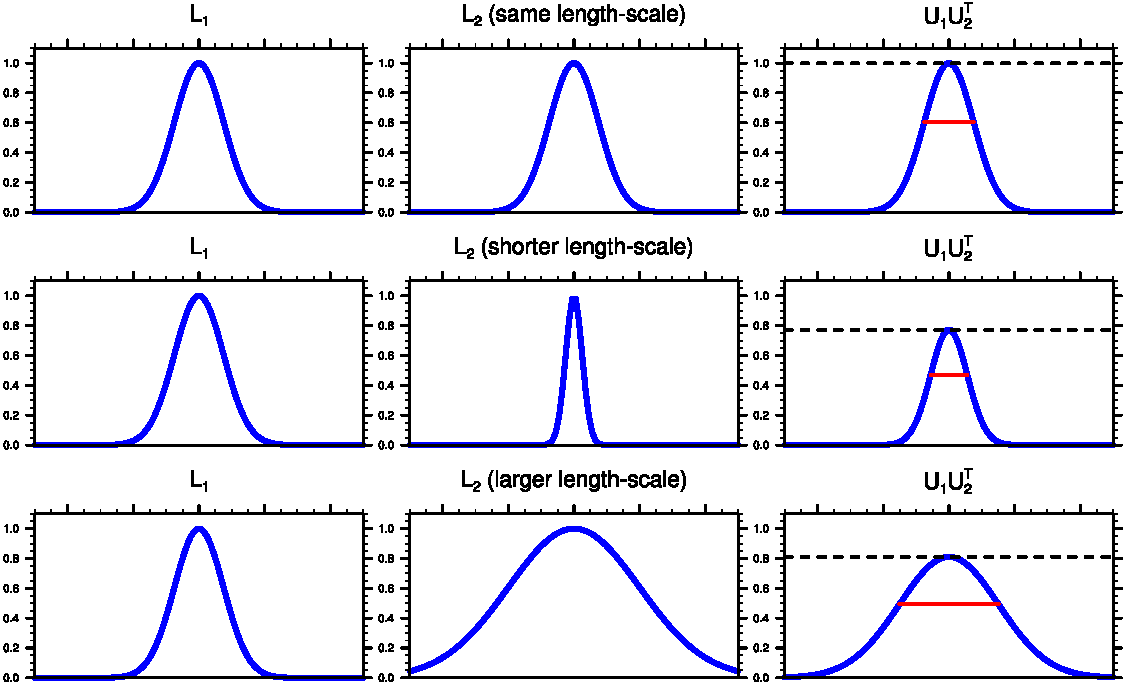
\includegraphics[width=\linewidth]{convolution_exp.pdf}
\captionof{figure}{1D illustration of the product of two localization square-root, with Gaussian localization functions. The dashed black line shows the function amplitude, while the solid red line shows the function length-scale.}
\end{center}

\section{Lower triangular square-root}

\subsection{General case}

\subsection{Same localization}
A fourth and final method defines $\mathbf{U}$ as:
\begin{align}
\mathbf{U} & = \mathbf{S}^\mathrm{s} \left( \begin{array}{cccc}
Q_{1,1} \overbar{\mathbf{U}} & 0 & \cdots & 0 \\
Q_{2,1} \overbar{\mathbf{U}} & Q_{2,2} \overbar{\mathbf{U}} & \ddots & \vdots \\
\vdots & \ddots & \ddots & 0 \\
Q_{p,1} \overbar{\mathbf{U}} & \cdots & Q_{p,p-1} \overbar{\mathbf{U}} & Q_{p,p} \overbar{\mathbf{U}}
\end{array} \right) \\
 & = \mathbf{S}^\mathrm{s} \left( \begin{array}{cccc}
Q_{1,1} \mathbf{I}_{\overbar{n}} & 0 & \cdots & 0 \\
Q_{2,1} \mathbf{I}_{\overbar{n}} & Q_{2,2} \mathbf{I}_{\overbar{n}} & \ddots & \vdots \\
\vdots & \ddots & \ddots & 0 \\
Q_{p,1} \mathbf{I}_{\overbar{n}} & \cdots & Q_{p,p-1} \mathbf{I}_{\overbar{n}} & Q_{p,p} \mathbf{I}_{\overbar{n}}
\end{array} \right) \left( \begin{array}{cccc}
\overbar{\mathbf{U}} & 0 & \cdots & 0 \\
0 & \overbar{\mathbf{U}} & \ddots & \vdots \\
\vdots & \ddots & \ddots & 0 \\
0 & \cdots & 0 & \overbar{\mathbf{U}} 
\end{array} \right)
\end{align}
where $\mathbf{I}_{\overbar{n}} \in \mathbb{R}^{\overbar{n} \times \overbar{n}}$ is the identity matrix. It should be noted that to apply $\mathbf{U}$, the matrix $\overbar{\mathbf{U}}$ needs to be applied $p$ times. The resulting localization matrix is:
\begin{align}
\mathbf{L} = \mathbf{U} \mathbf{U}^\mathrm{T} = \mathbf{S}^\mathrm{s} \left( \begin{array}{ccc}
W_{1,1} \overbar{\mathbf{U}} \overbar{\mathbf{U}}^\mathrm{T} & \cdots & W_{1,p} \overbar{\mathbf{U}} \overbar{\mathbf{U}}^\mathrm{T} \\
\vdots & \ddots & \vdots  \\
W_{p,1} \overbar{\mathbf{U}} \overbar{\mathbf{U}}^\mathrm{T} & \cdots & W_{p,p} \overbar{\mathbf{U}} \overbar{\mathbf{U}}^\mathrm{T}
\end{array} \right) \mathbf{S}^{\mathrm{s} \mathrm{T}}
\end{align}
where $\mathbf{W} = \mathbf{Q} \mathbf{Q}^\textrm{T}$. In this case, each auto- or cross-localization block is given by: 
\begin{align}
\mathbf{L}_{ij} = W_{i,j} \mathbf{S}^\mathrm{s}_i \overbar{\mathbf{U}} \overbar{\mathbf{U}}^\mathrm{T} \mathbf{S}_j^{\mathrm{s} \mathrm{T}}
\end{align}
The actual process would be reversed: first define $\mathbf{W}$, and its square-root decomposition $\mathbf{Q}$. Since $\mathbf{W}$ and $\mathbf{Q}$ are square matrices of size $p$, a Cholesky decomposition can work.\\
$  $\\
\textbf{Advantages:} precise control on the cross-localization amplitude.\\
\textbf{Drawbacks:} ill-adapted for large differences between variables length-scales.\\
\textbf{Cost:} $p$ applications of $\overbar{\mathbf{U}}$.

\subsection{Diagonal case}
A second method defines $\mathbf{U}$ as:
\begin{align}
\mathbf{U} = \left( \begin{array}{cccc}
\mathbf{U}_1 & 0 & \cdots & 0 \\
0 & \mathbf{U}_2 & \cdots & 0 \\
\vdots & \vdots & \ddots & \vdots \\
0 & 0 & \cdots & \mathbf{U}_p
\end{array} \right)
\end{align}
where $\mathbf{U}_i \in \mathbb{R}^{n_i \times m_i}$, $m_i$ being the size of the control sub-vector related to variable $i$ with $\displaystyle m = \sum_{i=1}^p m_i$. The resulting localization matrix is:
\begin{align}
\mathbf{L} = \mathbf{U} \mathbf{U}^\mathrm{T} = \left( \begin{array}{cccc}
\mathbf{U}_1 \mathbf{U}_1^\mathrm{T} & 0 & \cdots & 0 \\
0 & \mathbf{U}_2 \mathbf{U}_2^\mathrm{T} & \cdots & 0 \\
\vdots & \vdots & \ddots & \vdots \\
0 & 0 & \cdots & \mathbf{U}_p \mathbf{U}_p^\mathrm{T} 
\end{array} \right)
\end{align}
In this case, auto-localization blocks are well defined:
\begin{align}
\mathbf{L}_{ii} = \mathbf{U}_i \mathbf{U}_i^\mathrm{T}
\end{align}
but cross-localization blocks $\mathbf{L}_{ij}$ are zero for $i \ne j$.\\
$  $\\
\textbf{Control vector size:} $\displaystyle m = \sum_{i=1}^p m_i$.\\
\textbf{Cost:} one application of each $\mathbf{U}_i$.

\subsection{Block-diagonal case}
For the case where several variables share the same localization, a common localization $\mathbf{U}_\alpha \in \mathbb{R}^{n_\alpha \times m_\alpha}$ is defined for each group of variables $\alpha$, along with the concatenated matrix:
\begin{itemize}
\item $\widehat{\mathbf{U}}_\alpha \in \mathbb{R}^{n_\alpha p_\alpha \times m_\alpha}$:
\begin{align}
\widehat{\mathbf{U}}_\alpha = \left( \begin{array}{c}
\mathbf{U}_\alpha\\
\vdots \\
\mathbf{U}_\alpha
\end{array} \right)
\end{align}
\end{itemize}
The square-root $\mathbf{U}$ is defined as:
\begin{align}
\mathbf{U} = \left( \begin{array}{cccc}
\widehat{\mathbf{U}}_1 & 0 & \cdots & 0 \\
0 & \widehat{\mathbf{U}}_2 & \ddots & \vdots \\
\vdots & \ddots & \ddots & 0 \\
0 & \cdots & 0 & \widehat{\mathbf{U}}_q
\end{array} \right) = \left( \begin{array}{cccc}
\widehat{\mathbf{I}}_1 & 0 & \cdots & 0 \\
0 & \widehat{\mathbf{I}}_2 & \ddots & \vdots \\
\vdots & \ddots & \ddots & 0 \\
0 & \cdots & 0 & \widehat{\mathbf{I}}_q
\end{array} \right) \left( \begin{array}{cccc}
\mathbf{U}_1 & 0 & \cdots & 0 \\
0 & \mathbf{U}_2 & \ddots & \vdots \\
\vdots & \ddots & \ddots & 0 \\
0 & \cdots & 0 & \mathbf{U}_q
\end{array} \right)
\end{align}
The resulting localization matrix is:
\begin{align}
\mathbf{L} = \mathbf{U} \mathbf{U}^\mathrm{T} = \left( \begin{array}{cccc}
\widehat{\mathbf{U}}_1 \widehat{\mathbf{U}}_1^\mathrm{T} & 0 & \cdots & 0 \\
0 & \widehat{\mathbf{U}}_2 \widehat{\mathbf{U}}_2^\mathrm{T} & \ddots & \vdots \\
\vdots & \ddots & \ddots & 0 \\
0 & \cdots & 0 & \widehat{\mathbf{U}}_q \widehat{\mathbf{U}}_q^\mathrm{T}
\end{array} \right)
\end{align}
In this case, each auto- or cross-localization block within a group of variables ($G(i) = G(j)$) is given by: 
\begin{align}
\mathbf{L}_{ij} = \mathbf{U}_{G(i)} \mathbf{U}_{G(i)}^\mathrm{T}
\end{align}
but cross-localization blocks $\mathbf{L}_{ij}$ are zero for $G(i) \ne G(j)$ (variables of different groups).\\
$  $\\
\textbf{Control vector size:} $\displaystyle m = \sum_{\alpha=1}^q m_\alpha$.\\
\textbf{Cost:} one application of each $\mathbf{U}_\alpha$.

\clearpage

\bibliographystyle{mybib-en}
\bibliography{multivariate_localization}
\end{document}
